\documentclass [12pt]{article}
\usepackage{fancyhdr}
\usepackage[utf8]{inputenc}
\usepackage[english]{babel}
\usepackage{gensymb}
\usepackage{amsmath,amssymb,amsfonts}
\usepackage{algorithmic}
\usepackage{graphicx}
\usepackage{textcomp}
\usepackage[table]{xcolor}
\usepackage{siunitx}
\usepackage{indentfirst}
\usepackage[margin=2.5cm]{geometry}
\usepackage{float}
\usepackage{hyperref}
\usepackage[UKenglish]{datetime}
\usepackage{setspace}
\usepackage{hhline}
\usepackage{lastpage}
\usepackage[numbers]{natbib}
\usepackage[acronym]{glossaries}
\usepackage{listings}
\usepackage{color}
\usepackage{booktabs}% http://ctan.org/pkg/booktabs
\newcommand{\tabitem}{~~\llap{\textbullet}~~}
\usepackage{subfigure}

\usepackage{helvet}
\renewcommand{\familydefault}{\sfdefault}

\definecolor{customgreen}{rgb}{0,0.6,0}
\definecolor{customgray}{rgb}{0.5,0.5,0.5}
\definecolor{custommauve}{rgb}{0.6,0,0.8}

\graphicspath{{images/}}

\hypersetup
{
    colorlinks=true,
    linkcolor=black,
    urlcolor=blue,
    citecolor=black,
}

\doublespacing

\begin{document}

\title{\bf IP Landscape}
\author{Daniel Cole, Jack Pendlebury, Noah Harvey, Luke Waller}
\date{\today}

\begin{titlepage}
    \begin{center}
        \vspace*{1cm}

        \vspace*{\baselineskip}

        \rule{\textwidth}{1.6pt}\vspace*{-\baselineskip}\vspace*{2pt}
        \rule{\textwidth}{0.4pt}\\

        {\LARGE IP\\ [0.3\baselineskip] Landscape}\\[0.2\baselineskip]

        \rule{\textwidth}{0.4pt}\vspace*{-\baselineskip}\vspace{3.2pt}
        \rule{\textwidth}{1.6pt}\\[\baselineskip]
        \scshape

        \textbf{Daniel Cole, Jack Pendlebury, Noah Harvey, Luke Waller}

        \today

        \vfill

        IP landscape for the HEVCS platform.

        \vspace{0.8cm}

        
\includegraphics[width=0.4\textwidth]{UOP_Logo.png}

    \end{center}
\end{titlepage}

\newpage
\fancyfoot[R]{Page \thepage \hspace{1pt} of \pageref{LastPage}}
\setcounter{page}{1}
\pagenumbering{arabic}
\tableofcontents
\newpage

\listoffigures
\listoftables

\newpage
\section{Patent Landscape Analysis}\label{sec:PLA}

A patent is a form of intellectual property that provides the legal owner with exclusive rights to the invention.
This prevents others from using, making, and selling the invention while the patent is in force.
New patents can only be filed for new, useful, and novel inventions that contain patentable subject matter.
In 2020 there were over 16 million patents in force worldwide \cite{WIPO_ref}.
Corporations wishing to develop innovative products are faced with the challenge of critically analysing the patents within their proposed patent scope.
Prior art is a concept within patent law that is used to determine whether the product is patentable or not.
The purpose of the landscape is to ensure that the patent applicant will not infringe on prior art, and that the invention is in fact novel and unique.

\section{Project Overview}\label{sec:project_overview}
\subsection{Project Details}\label{sec:project_details}

The Home Electric Vehicle Charging System (HEVCS) provides a means to charge an electric vehicle for those without adequate space to install charging equipment at home, whilst easing the strain on existing charging infrastructure.
Given that the majority of UK homes within cities lack dedicated parking, an electric vehicle (EV) becomes a less desirable option for personal use.
These issues arrise when using a standard plug-in system to charge their EV from their home.
There are significant logistcal problems that arise from trying to charge vehicles when not near the users home, such as lack of public charging infrastructure and having to use large cables that would run across the pavement.
\\
To solve this problem, HEVCS provides a platform that allows a user to charge their vehicle without a permanent installation.
When not in use, the platform will charge at the user's home, with options for indoor or outdoor installation.
When the user requires their car to be charged, they will remotely drive the platform from their home to under their vehicle, where be connected to the car and initiate charging.
By fitting under a user's vehicle, the HEVCS platform will reduce the curbside footprint but will act as a deterrent to theft.
\\
The HEVCS platform will be able to provide enough power to charge half the capacity of a small EV such as the Nissan Leaf.
This has been done to reduce costs and allow the platform to fit under the vehicle whilst charging.
For the majority of vehicles, this will provide enough range to perform a user's morning commute, where they may be able to access a better equipt charging point.

\subsection{Inspiration}\label{sec:inspiration}

The team working on HEVCS shares a love of motor vehicles, all the way from motorsport to classic car restoration and repair.
The team agrees that EVs are the future and to pretend otherwise would be missing a huge market opportunity.
As young professionals encumbered by the rising cost-of-living, and volatile cost of traditional vehicle fuels, they would be an intended market for the new ranges of low-cost hatchback-style EVs, designed for city commutes.
However, there is a significant lack of charging facilities, especially within UK based short-term housing.

\subsection{Intended Market}\label{sec:intended_market}

As in most housing markets, there is a significant overlap between those driving small EVs for daily commutes and those people that do not own housing with driveways \cite{Home_Chargepoints}.
For this reason, the cost must be kept competitive.
It is hoped that the eventual product would be able to be included in the cost of a car, perhaps as a package deal from the dealership.
Even so, the cost of the final unit would be reasonable for someone purchasing a small-sized EV (£5000).

\subsection{Safety and Ethical Considerations}\label{sec:SAEC}

To both comply with legislation and to aid in ease-of-use, the platform will contain a full suite of safety features to minimise the risk of harm to the user, the user's property, any members of the public nearby, and property belonging to any third parties.
The platform will be semi-autonomous, handling critical tasks such as step and kerb navigation on the user's behalf.
The charging cells used will be second-hand, reducing costs and helping to mitigate some of the severe environmental effects of lithium extraction.

\subsection{Market Competition}\label{sec:market_competition}

Current solutions to the problem of charging EVs are currently lacking in several key areas.
The idea of converting streetlamp circuits to provide the requisite power to charge an EV is difficult, as much of the circuitry must be replaced and streets dug up.
To convert every streetlamp within a city would have an inordinate cost and would cause extreme delays throughout the city.
Relying solely on workplaces to provide charging points also disadvantages small businesses and those that work at said businesses, who lack private parking or even the space to provide charging facilities.
HEVCS seeks to mitigate these issues as much as possible, by providing a means to provide at least partial charging to those without guaranteed parking.
\\
As EVs become ever more prolific, and more legislation is bought in to ban the sale of new internal combustion engine powered vehicles, solutions to the charging problem will become more and more important.
While the burden of a nationwide need for a solution will be too great for this one platform to bear, it will be the first amongst many.

\subsection{Design Requirements}\label{sec:design_requirements}

The scope of the project has been defined by the following requirements:
\begin{enumerate}
    \item The platform must abide by class 2 mobility scooter legislation and the respective highway regulations to be road legal.
    \item The platform must be able to navigate the home, roads and pavements and the relevant obstacles such as kerbs and a maximum of three steps while transporting the payload from the user's home to their car.
    \item The platform must be always controlled by the user via a tethered connection to move. Upon disconnection, the device enters an immobilised state.
    \item The robot must be capable of acknowledging hazards, such as too steep a slope, too many steps and obstructions. In these cases, the robot must refuse to tackle such obstacles and override the user's inputs.
    \item The platform must be stored safely within the docking station that minimises the space in which it occupies whilst it charges the EV battery.
    \item The platform must be able to drive underneath EV's with a ground clearance of 155mm and above and lock itself securely to the vehicle.
    \item The platform will not attempt to traverse inclines/declines greater than 20 degrees.
  \end{enumerate}


\section{HEVCS Key Constituent Parts}\label{sec:constituent_parts}

\subsection{Under Vehicle Technology}

One of the most important features of the device is that it can fit underneath electric vehicles. To determine the maximum dimensions of the platform, data was gathered to analyse trends in ground clearance. This data is documented in the electric vehicle dimensions spreadsheet. The data set used contained 34 of the most common EVs, their respective ground clearance and battery capacity. To summarise, a platform with a maximum height of 150mm would fit beneath 53\% of the EVs.

The platforms key design characteristics include a chassis consisting of aluminium extrusion, corner plates and various nuts and bolts. Mounted to the chassis will have four driven and two passive wheels. In addition to these, two arms will be attached to the front of the carriage to traverse up and down steps.

The platform will transport the mechanical propulsion equipment and electronics, as well as the payload of the EV battery. The power will be sourced from rechargeable golf caddy batteries with the appropriate adapters to power motors and electrical equipment independently. Each system has been designed to be modular and operate independently, while communicating with each one another.

\begin{figure}[h]
    \centering
    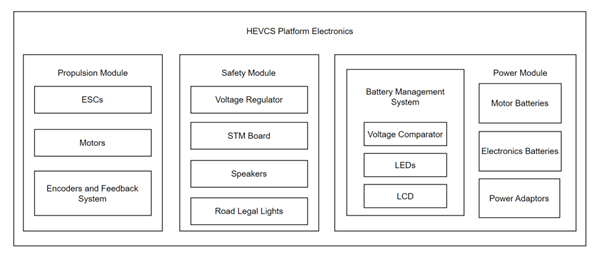
\includegraphics[width = 8cm]{PlatformHardware.png}
    \caption{HEVCS Platform Electronic Systems Diagram}
\end{figure}

The propulsion system will utilise pulleys and gear boxes to increase the torque of the motors to aid their intended use. Additional arms will be mounted to the chassis to assist the system with traversing steps. These motors will control wheels that can be manipulated to overcome edges and angles.

The safety module serves to fulfil the lighting and alarm requirements for the platform to be road legal. The battery management system will display the information about the current capacity of the platform’s battery and the EV battery it will carry. The propulsion module is used to control the motors to transport the carriage from the user’s home to the EV.

The power module includes the batteries that power the motors and electronics within different modules using appropriate power adapters. The battery management system will measure the capacity of the batteries mounted within the platform, and the payload battery. The payload battery is used to charge the EV’s battery. Serial communication will be used between the different modules inside the HEVCS, as well as with the controller. 

Both the payload battery and the system battery are charged within the home from the mains plug. The system battery, which powers the motors and electrical equipment, is also charged from home mains power and is not connected to the payload battery. The user is required to switch on the mains power and connect a cable to the HEVCS platform.

The system interfaces with the EV in a physical manner only. There are no wireless connections or communications to or from the HEVCS platform. The first physical connection is from the payload battery to the EV’s battery, which is done by the user with an off the shelf charging cable. The payload battery can then transfer its charge to the EV’s battery. The controller interfaces with the platform through a magnetic breakaway cable that the user must also connect themselves. The platform will not move if this controller is not connected, disconnection during operation results in immobilisation. The controller is powered via the cabled connection from the HEVCS.

Brackets will be included in the design to provide users options for additional security measures, such as chains or clamps, which will be off the shelf products for mounting mechanisms such as the towing anchor for the car. They will not interface with the electronics of the HEVCS platform or the EV itself.

The arrears for patent research have been determined as devices that are capable of going underneath vehicles, platforms capable of traversing kerb/steps and platforms capable of charging EV’s.

\subsection{Magnetic Breakaway Cable}

The magnetic breakaway cable connector will feature a magnetic design, using a single lug to control the rotation of the connector. The cable will be male-to-male, with a ten-pin connector at each end. Each pin will be a spring-loaded pogo-pin, ensuring quality of connection. The prototype connector housing will be 3D printed.

The pins will be arranged in a circular manner around the central magnet. The magnets at each end will be connected, to act as a ground. The ten pins will be allocated thusly:

\begin{table}[H]
    \centering
    \setlength{\arrayrulewidth}{1.5pt}
    \begin{tabular}{|p{0.7\linewidth}|c|}
    \hline
    \cellcolor{gray!40}Allocation & \cellcolor{gray!40}No. of Pins\\
    \hline
    SPI Bus 0 & 3 \\
    \hline
    SPI Bus 1 & 3 \\
    \hline
    Controller Connection Detect & 1 \\
    \hline
    Unallocated & 3 \\
   \hline
    \end{tabular}
    \caption{Breakaway Pin Allocations}
    \label{table:breakaway_pin_allocations}
\end{table}

The unallocated pins could be used for an additional SPI bus, or alternatively to provide power for the controller if battery power is not used.

The connection will be maintained using the strength of the central magnets. Should the HEVCS platform get too far away from the user, such as in event of a drive failure or incapacitation of the user, the force will disconnect the controller. This will trigger the safety protocols of the platform, immobilising it.

The female connector will be made with PCB pads as the contacts, arranged circularly around a magnet. This magnet will be grounded, to be used as the ground in the connector wire. The cable will be wrapped in a PVC mesh to provide durability.

\section{Patent Research}\label{sec:patent_research}
When performing research into the IP landscape surrounding a project, it is important to filter patents to only include relevant results. As one of leading patent databases, Espacenet was used to find patents. One of the most helpful features of Espacenet is the advanced search features available, with support for Boolean logic as well as filtering based on report section.

These features were used liberally, with each search strategy making use of Boolean OR statements to include equivalent terms or variants of a word. Given that a large number of patents are translated into English, alternate word choices were important as translations are not always optimal. Another filtering method was to filter based on words within the title; title and abstract; or all text within the document. This helped to further filter results by ignoring uses of words in non-relevant sections. In some cases, an exclusionary NOT term was added, to ignore specific terms that appeared in non-relevant results.

The objective of each search was to lower the number of relevant results to approximately ten, and then to survey the results in detail for any risk of infringement.

\subsection{Under Vehicle Technology}\label{sec:under_vehilce_technology}

\subsubsection{Search Strategies}

The advanced search tool was used to locate the following phrases in the title or abstract. The phrases started with list various words related to how the technology would be placed under a vehicle to develop an understanding of the language used in existing patents. Then, the use of the bitwise OR function was used when multiple words and phrases were used to describe existing technology.

\subsubsection{Search Strategy 1}

\begin{table}[H]
    \centering
    \setlength{\arrayrulewidth}{1.5pt}
    \begin{tabular}{|p{0.7\linewidth}|c|}
    \hline
    \cellcolor{gray!40}Search Term & \cellcolor{gray!40}No. of Results \\
    \hline
    ta any “carriage” AND ta any “underneath vehicle” & 28,241 \\
    \hline
    ta any “platform” AND ta any “underneath vehicle” & 2,030 \\
    \hline
    (ta any “platform” OR ta any “carriage”) AND ta any “under electric vehicle” & 266,484 \\
    \hline
    (ta any “platform” OR ta any “carriage”) AND ta any “under electric vehicle” AND ta any “electric vehicle” & 179,323 \\
    \hline
    (ta any “platform” OR ta any “carriage”) AND ta any “under vehicle” AND ta any “electric vehicle” & 105,202 \\
    \hline
    (ta any “platform” OR ta any “carriage”) AND ta any “underneath electric vehicle” AND ta any “electric vehicle” & 179,323 \\
    \hline
    \end{tabular}
    \caption{Under Vehicle Technology Search Terms 1}
    \label{table:under_vehicle__search_strat_1}
\end{table}

The search strategy continued to use the phrase “under electric vehicle” rather than “under vehicle” and it returned more results and was more relevant to the project. Altering the phrase to say “underneath electric vehicle” had no effect on the patents returned.

\subsubsection{Search Strategy 2}

\begin{table}[H]
    \centering
    \setlength{\arrayrulewidth}{1.5pt}
    \begin{tabular}{|p{0.7\linewidth}|c|}
    \hline
    \cellcolor{gray!40}Search Term & \cellcolor{gray!40}No. of Results \\
    \hline
    (ta any “platform” OR ta any “carriage”) AND ta any “underneath electric vehicle” AND ta any “charge” & 3,059 \\
    \hline
    (ta any “platform” OR ta any “carriage”) AND ta any “underneath electric vehicle” AND ta any “charge” AND ta any “electric vehicle” & 3,078 \\
    \hline
    (ta any “platform” OR ta any “carriage”) AND ta any “underneath electric vehicle” AND ta any “charge” AND ta any “user driven” & 538 \\
    \hline
    (ta any “platform” OR ta any “carriage”) AND ta any “under electric vehicle” AND ta any “charge” AND ta any “electric vehicle” AND ta any “user driven” & 528 \\
    \hline
    (ta any “platform” OR ta any “carriage”) AND ta any “under electric vehicle” AND ta any “charge” AND ta any “electric vehicle” AND ta any “manned” & 2 \\
    \hline
    \end{tabular}
    \caption{Under Vehicle Technology Search Terms 2}
    \label{table:under_vehicle__search_strat_2}
\end{table}

The phrase “manned” was too specific and returned patents where the platforms were intended for use underwater. The HECVS will not go underwater, and so there is no potential for infringement of these patents. The search term was then returned to the original phrase of “user driven”.

\subsubsection{Search Strategy 3}

\begin{table}[H]
    \centering
    \setlength{\arrayrulewidth}{1.5pt}
    \begin{tabular}{|p{0.7\linewidth}|c|}
    \hline
    \cellcolor{gray!40}Search Term & \cellcolor{gray!40}No. of Results \\
    \hline
    (ta any “platform” OR ta any “carriage”) AND ta any “under electric vehicle” AND ta any “charge” AND ta any “electric vehicle” AND ta any “user driven” AND ta any “remote control” & 182 \\
    \hline
    (ta any “platform” OR ta any “carriage”) AND ta any “under electric vehicle” AND ta any “charging” AND ta any “electric vehicle” AND ta any “manned” AND ta any “remote control” & 447 \\
    \hline
    \end{tabular}
    \caption{Under Vehicle Technology Search Terms 3}
    \label{table:under_vehicle_search_strat_3}
\end{table}

There was a large difference in the number of results returned depending on whether the phrase “charge” or “charging” was used, so the search field was updated to return patents containing either phrase.

\subsubsection{Search Strategy 4}

\begin{table}[H]
    \centering
    \setlength{\arrayrulewidth}{1.5pt}
    \begin{tabular}{|p{0.7\linewidth}|c|}
    \hline
    \cellcolor{gray!40}Search Term & \cellcolor{gray!40}No. of Results \\
    \hline
    (ta any “platform” OR ta any “carriage”) AND (ta any “charge” OR ta any “charging”) AND ta any “under electric vehicle” AND ta any “electric vehicle” AND ta any “user driven” AND ta any “remote control” & 537 \\
    \hline
    (ta any “platform” OR ta any “carriage”) AND (ta any “charge” OR ta any “charging”) AND ta any “under electric vehicle” AND ta any “electric vehicle” AND ta any “user driven” AND ta any “remote control” AND ta any “battery” & 148 \\
    \hline
    (ta any “platform” OR ta any “carriage”) AND (ta any “charge” OR ta any “charging”) AND ta any “under electric vehicle” AND ta any “electric vehicle” AND ta any “user driven” AND ta any “remote control” AND ta any “load” & 12 \\
    \hline
    (ta any “platform” OR ta any “carriage”) AND (ta any “charge” OR ta any “charging”) AND ta any “under electric vehicle” AND ta any “electric vehicle” AND ta any “user driven” AND ta any “remote control” AND ta any “load carrying” & 21 \\
    \hline
    \end{tabular}
    \caption{Under Vehicle Technology Search Terms 4}
    \label{table:under_vehicle_search_strat_4}
\end{table}

The search term “load carrying” returned nine more results that “transporting” and “bearing”, showing that the generalised term for transporting a load was more widely used. When the search term was altered to return results with either the “load carrying” or “load” mentioned within the title or abstract, the number of results returned was still 21. The single worded phrase “load” was sufficient in identifying relevant patents with the correct intended use.


\textbf{Final Search Term}

\begin{table}[H]
    \centering
    \setlength{\arrayrulewidth}{1.5pt}
    \begin{tabular}{|p{0.7\linewidth}|c|}
    \hline
    \cellcolor{gray!40}Search Term & \cellcolor{gray!40}No. of Results \\
    \hline
    ta any “under electric vehicle” AND (ta any “platform” OR ta any “carriage”) AND ta any “electric vehicle” AND ta any “remote control” AND (ta any “charging” OR ta any “charge”) AND ta any “stationary vehicle” AND ta any “user driven” AND ta any “load” AND ta any “battery” & 8 \\
    \hline
    \end{tabular}
    \caption{Under Vehicle Technology Final Search Terms}
    \label{table:under_vehicle_final_search_strat}
\end{table}

\subsubsection{Patent 1 - Electric Automobile Monitored Control System based on Cloud Platform}

\begin{table}[H]
    \centering
    \setlength{\arrayrulewidth}{1.5pt}
    \begin{tabular}{|p{0.5\linewidth}|p{0.5\linewidth}|}
    \hline
    Patent Number & \href{https://worldwide.espacenet.com/patent/search/family/059570588/publication/CN206422800U?q=pn%3DCN206422800U}{CN206422800U}\\
    \hline
    Applicants & GUANGXI YULIN GUANGNENG ELECTRONIC TECH CO LTD\\
    \hline
    Status & ACTIVE, GRANTED 18/08/2017\\
    \hline
    Application Date/Publish Date & 03/02/2017 / 18/08/2017\\
    \hline
    Active Jurisdictions & CHINA \\
    \hline
    \end{tabular}
    \caption{Under Vehicle Technology - Patent 1 Information}
    \label{table:under_vehicle_patent_1}
\end{table}
\textbf{Independent Claims Analysis}\\
This patent covers an electric vehicle monitoring system that collates real-time electricity prices. The data is stored on cloud-based storage, detailed in the patent’s single independent claim.

\textbf{Independent Claim 1}\\
The single independent claim states that the monitoring system has a cloud server connected to the data grid. The HEVCS will not collect, or store data related to the user’s electric vehicle or electricity prices, therefore there is no permanent database required either. The HEVCS will not contain a data control unit either.

\textbf{Independent Claims Summary}\\
As stated in the review of independent claim, the HEVCS does not track, store or present data obtained from monitoring EVs or electricity prices. In addition to this, the patent is only active in China, therefore, there is no infringement upon this patent.

\subsubsection{Patents 2 and 3 - Patent Family - Charging and Discharging System}

\begin{table}[H]
    \centering
    \setlength{\arrayrulewidth}{1.5pt}
    \begin{tabular}{|p{0.5\linewidth}|p{0.5\linewidth}|}
    \hline
    Patent A Number & \href{https://worldwide.espacenet.com/patent/search/family/050051436/publication/CN103580250A?q=pn%3DCN103580250A}{CN103580250A}\\
    \hline
    Patent B Number & \href{https://worldwide.espacenet.com/patent/search/family/050051436/publication/CN103580250B?q=CN103580250B}{CN103580250B}\\
    \hline
    Applicants & GUANGXI YULIN GUANGNENG ELECTRONIC TECH CO LTD CHERY AUTOMOBILE CO LTD \\
    \hline
    Status & ACTIVE, GRANTED 27/04/2016 \\
    \hline
    Application Date/Publish Date of Patent A & 31/10/2013 / 12/02/2014 \\
    \hline
    Application Date/Publish Date of Patent B & 31/10/2013 / 27/04/2016 \\
    \hline
    Active Jurisdictions & CHINA \\
    \hline
    \end{tabular}
    \caption{Under Vehicle Technology - Patents 2 and 3 Information}
    \label{table:under_vehicle_patent_2and3}
\end{table}

\textbf{Independent Claim Analysis}\\
There are five independent claims that are identical in both the patents within this family.

\textbf{Independent Claim 1}\\
The first claim states that a touch screen is used as the human interface to provide instructions to the platform. The HEVCS will not contain a touch screen, instead the user can operate the platform with a bespoke controller.

\textbf{Independent Claim 2}\\
This claim states the charge/discharge control system contains a power price analysis module with the ability for the user to submit their own commands.  The HEVCS will not monitor the price of power and will not contain a smart grid interactive scheduling platform.

\textbf{Independent Claim 3}\\
This claim mentions that the system is mounted onto vehicles while communicating with the power grid wirelessly. The HEVCS will not have any form of wireless communication and will not communicate with the grid by other means. The platform itself, and systems within, will not be attached to the vehicles. The only contact made is between the platform’s payload, being the battery carrying the charge, and the vehicle’s battery.

\textbf{Independent Claim 8}\\
This claim discusses the methods used to predict when the EV should charge or discharge. An algorithm determines when the system stops charging or discharging both the EV and power grid. The HEVCS will charge payload and system batteries when the user plugs the system into a socket at the platform’s charging station. There will be no algorithms or user inputs that allow for a pre-set period of charging. The system will stop charging when the user switches off the mains power supply or the batteries have reached full capacity.

\textbf{Independent Claim 9}\\
This claim further details the methods used for pre-set timing intervals of charging the EV. It states that the upper charge and discharge limits, from power grid to EV battery, are limited. The HEVCS will not connect the power grid directly to the EV.

\textbf{Independent Claims Summary}\\
The above independent claims for both patents share the same feature of the system relating to the power grid being connected directly to the EV. As the HEVCS will not charge the EV battery in this manner, as it provides a payload battery to EV battery connection only. It must also be recognised that while the HEVCS platform charges, by being connected to the power grid, it is not tracking the price of power or storing any data related to electricity usage. In summary, the HEVCS does not infringe on this active patent due to its differences in design and application, as well as the patent itself only being in force in China.

\subsubsection{Patent 4 - Intelligent Electricity Charging and Alternating System Based on Cloud Platform}

\begin{table}[H]
    \centering
    \setlength{\arrayrulewidth}{1.5pt}
    \begin{tabular}{|p{0.5\linewidth}|p{0.5\linewidth}|}
    \hline
    Patent Number & \href{https://worldwide.espacenet.com/patent/search/family/059446220/publication/CN107009911A?q=pn%3DCN107009911A}{CN107009911A}\\
    \hline
    Applicants & UNIV GUIZHOU \\
    \hline
    Status & NOT ACTIVE, SEARCH AND EXAMINATION 29/08/2017 \\
    \hline
    Application Date/Publish Date & 10/04/2017 / 04/08/2017 \\
    \hline
    Active Jurisdictions & CHINA \\
    \hline
    \end{tabular}
    \caption{Under Vehicle Technology - Patent 4 Information}
    \label{table:under_vehicle_patent_4}
\end{table}

\textbf{Independent Claim Analysis}\\
The patent has a single independent claim featuring various characteristics that the HEVCS does not possess.

\textbf{Independent Claim 1}\\
The single independent claim states that the device uses an intelligent charging system which is cloud based, with both wired and wireless connection to the charging pile. The cloud platform can also be accessed with a mobile phone app. The HEVCS will not have any wireless connections or collect and store any data, and so there is no cloud-based platform either.

\textbf{Independent Claims Summary}\\
As the single independent claim consists of multiple features that the HEVCS will not possess, it would not infringe upon this patent if it were approved and becomes active in the same jurisdiction.

\subsubsection{Patent 5 - Scheduling System and Method for Stabiliizing Transformer Substation}
\begin{table}[H]
    \centering
    \setlength{\arrayrulewidth}{1.5pt}
    \begin{tabular}{|p{0.5\linewidth}|p{0.5\linewidth}|}
    \hline
    Patent Number & \href{https://worldwide.espacenet.com/patent/search/family/071428323/publication/CN111404168A?q=pn%3DCN111404168A}{CN111404168A} \\
    \hline
    Applicants & UNIV CHONGQING POSTS and TELECOM \\
    \hline
    Status & NOT ACTIVE, SEARCH AND EXAMINATION 04/08/2020 \\
    \hline
    Application Date/Publish Date & 09/12/2019 / 10/07/2020 \\
    \hline
    Active Jurisdictions & CHINA \\
    \hline
    \end{tabular}
    \caption{Under Vehicle Technology - Patent 5 Information}
    \label{table:under_vehicle_patent_5}
\end{table}

\textbf{Independent Claim Analysis}\\
This patent has one individual claim that states how the dispatch system collects data from power grids to monitor the effects of electric vehicle’s cabin temperatures.

\textbf{Independent Claim 1}\\
The cloud monitoring system receives and displayed the operational data of electric vehicles, charging stations, substations, and users. The data obtained includes temperatures and their respective cruising ranges, combining the statistics to measure and predict efficiency. To measure the cruising range the system has access to the location of every electric vehicle it is installed in. This location data is collated to produce heat maps that highlight electric vehicle hot spots. The HEVCS does not take temperature readings of the electric vehicle or collect information from any pre-existing charging infrastructure. It will not track the location of the vehicle, as it will only be driven underneath stationary vehicles.

\textbf{Independent Claims Summary}\\
The independent claim details multiple features which the HEVCS does not have, and data that it will not obtain. In summary, if this patent became active in the same jurisdiction, the HEVCS project would not infringe this patent.

%%%%%%%%%%% END OF 5
\subsubsection{Patent 6 - Multi-Energy-Source Crawler-Type Electric Drive Platform for Grassland Unmanned Inspection}

\begin{table}[H]
    \centering
    \setlength{\arrayrulewidth}{1.5pt}
    \begin{tabular}{|p{0.5\linewidth}|p{0.5\linewidth}|}
    \hline
    Patent Number & \href{https://worldwide.espacenet.com/patent/search?q=pn%3DCN210821848U}{CN210821848U}\\
    \hline
    Applicants & UNIV INNER MONGOLIA TECHNOLOGY \\
    \hline
    Status & NOT ACTIVE, TERMINATED 18/10/2022 \\
    \hline
    Application Date/Publish Date & 06/11/2019 / 23/05/2020 \\
    \hline
    Active Jurisdictions & CHINA \\
    \hline
    \end{tabular}
    \caption{Under Vehicle Technology - Patents 6 and 7 Information}
    \label{table:under_vehicle_patent_6}
\end{table}

\textbf{Independent Claim Analysis}\\
This patent has one independent claim that states the electronic systems within the design, and how they are connected.

\textbf{Independent Claim 1}\\
The claim starts by stating that the crawler has multiple energy sources, including solar power, that can provide power to the drive system. Further details discuss the fact that the crawler is unmanned while it carries out the intended use of inspecting grassland. The HEVCS is only powered by one form of energy, stored in the systems battery, having charged through a connection to a mains supply. The HEVCS is not an unmanned vehicle, and will not inspect grassland in the same manner as this crawler in the patent. The only purpose of the HEVCS inspecting its surroundings is to acknowledge the distance between the platform and surrounding objects, which could be on a patch of grassland. It does not inspect the grassland itself.

\textbf{Independent Claims Summary}\\
The power sources and intended use of the patents system are dissimilar from the energy source the HEVCS platform uses, and the information the LiDAR will obtain from the surroundings. For these reasons, if the patent were still active and in the same jurisdiction, the HEVCS would not infringe upon it.

\subsubsection{Patents 7 and 8 - Patent Family - Internet-Based Grid Connection Type Microgrid Joint Energy Management and Control Method}

\begin{table}[H]
    \centering
    \setlength{\arrayrulewidth}{1.5pt}
    \begin{tabular}{|p{0.5\linewidth}|p{0.5\linewidth}|}
    \hline
    Patent A Number & \href{https://worldwide.espacenet.com/patent/search/family/048437563/publication/KR20130035820A?q=KR20130035820A}{KR20130035820A}\\
    \hline
    Patent B Number & \href{https://worldwide.espacenet.com/patent/search/family/048437563/publication/KR101460488B1?q=pn%3DKR101460488B1}{KR101460488B1}\\
    \hline
    Applicants & PAC TECH CO LTD \\
    \hline
    Status & ACTIVE\\
    \hline
    Patent A Application Date/Publish Date & 03/09/2011 / 09/04/2013\\
    \hline
    Patent B Application Date/Publish Date & 30/09/2011 / 12/11/2014\\
    \hline
    Active Jurisdictions & KOREA \\
    \hline
    \end{tabular}
    \caption{Under Vehicle Technology - Patents 7 and 8 Information}
    \label{table:under_vehicle_patent_7and8}
\end{table}

\textbf{Independent Claim Analysis}\\
The first patent of the family has two independent claims, where the first focuses on monitoring apparatus   . The independent claims in the second patent build upon the first, and so they have been analysed together.

\textbf{Independent Claim 1}\\
The first independent claim is the same for each patent, with one containing more detail at a component level. Both are reviewed in this analysis. The claims state that the system includes an analysis unit for analysing the charging data it has collected while charging the vehicle. The data stored includes tracking information, which is downloaded and manipulated to display an overview of the progress of the charging routine. This is displayed to the user. This approach to monitoring the current charging capacity of the EV’s battery is the same as the HEVCS’s, but the difference lies with the information being stored. The HEVCS will not save the charging procedures data as a progressive figure over time. It will only display the current ‘live’ charging data to the user. The information will not be analysed once a reading is taken.

\textbf{Independent Claim 14}\\
The second patent in the family contains the definition of this claim, whereas the first does not. It states that the control unit reads a temperature value from the battery via the adjacent power-train control unit. If a failure was to occur, the power-train control unit can still retrieve temperature readings when the battery’s sensing unit cannot.

The HEVCS will measure the temperature of the individual units within the platform where a high temperature could indicate a failure or fault in the system. This includes the battery management unit for the motor battery, the payload battery while it charges the car and is charged within the home. The charging apparatus will also house temperature monitors. This array of sensing equipment will serve the same purpose of monitoring the battery, but is different to the patent in that it does not just record the temperature of the units performing the charging. The HEVCS needs temperature readings from other equipment, or batteries serving other functions to operate additional.

\textbf{Independent Claim 15}\\
A battery management unit comprising of charging and the necessary control apparatus. This claim is based on the control step, where the charger is switched off upon detecting a full charge. The control unit is separate to the charging unit. The status of the control unit is displayed, and the operational data is tracked. An analysis of its operation is then provided. The HEVCS will combine off the shelf charging equipment and batteries with these features built in, for both the unit that monitors both the payload and system battery in a similar manner.

\textbf{Independent Claims Summary}\\
The battery management system, and the charge control unit within, detailed in this patent is has similar applications as the HEVCS. The differences being that the independent claims 1 and 14 state that data obtained is stored and then further analysed. The patents within this family is not infringed upon, even if it were to apply to the same jurisdiction, as there are substantial differences between the data handling in this patent and the HEVCS.

\subsubsection{Patents 9 and 10 - Patent Family - Internet-Based Grid Connection Type Microgrid Joint Energy Management and Control Method}

\begin{table}[H]
    \centering
    \setlength{\arrayrulewidth}{1.5pt}
    \begin{tabular}{|p{0.5\linewidth}|p{0.5\linewidth}|}
    \hline
    Patent A Number & \href{https://worldwide.espacenet.com/patent/search/family/061753019/publication/CN107872068A?q=pn%3DCN107872068A}{CN107872068A}\\
    \hline
    Patent B Number & \href{https://worldwide.espacenet.com/patent/search/family/061753019/publication/CN107872068B?q=CN107872068B}{CN107872068B}\\
    \hline
    Applicants & STATE GRID SHANGHAI MUNICIPAL ELECTRIC POWER CO \\
    \hline
    Status & ACTIVE\\
    \hline
    Patent A Application Date/Publish Date & 29/09/2017 / 03/04/2018 \\
    \hline
    Patent B Application Date/Publish Date & 29/09/2017 / 09/02/2021 \\
    \hline
    Active Jurisdictions & CHINA \\
    \hline
    \end{tabular}
    \caption{Under Vehicle Technology - Patents 9 and 10 Information}
    \label{table:under_vehicle_patent_9and10}
\end{table}

\textbf{Independent Claim Analysis}\\
This patent family of two has one independent claim that is developed in the second patent, adding the project’s expansions.

\textbf{Independent Claim 1}\\
The system is comprised of an internet-based management joint, connecting to the grid and other renewable energy sources. It collects data to carry out load forecasting. The second patent states that there is an internet-based grid between users, sharing their details to encourage others to opt into the program. The second patent’s version of the independent claim details the user’s requirement to subscribe to take part in the next periods energy distribution plan which is shared on an internet-based platform. The HEVCS is not going to connect to the grid, or other energy sources, to obtain the data required for load forecasting. It will only connect to mains power sockets to charge the batteries.

\textbf{Independent Claims Summary}\\
The HEVCS will not share information between users, or use an internet-based platform, and so this patent would not be infringed upon if it were active in the same jurisdiction.



%%%%%%%%%%%%%%%%%%%%%%%%%%%%%%%%%%%%%%%%%%%%%%%%%%%
%%%%%%%%%%%%%%%%%%%%%%%%%%%%%%%%%%%%%%%%%%%%%%%%%%%

\subsection{Breakaway Connectors}\label{sec:breakaway_connectors}
\subsubsection{Search Strategies}
\textbf{Strategy 1}\\
Using the advanced search functionality of espacenet to filter results based on a search terms inclusion in just the title, the phrase “magnetic” and “break away” was used and returned a single patent.
Similar combinations with less strict filters returned more results, with “parallel” AND “cable” AND “magnetic” returning 29 results. \\
\textbf{Strategy 2}\\
An alternate strategy was attempted, by placing emphasis on the break-away/pull-apart functionality of the connector. This led to the following results:

\begin{table}[H]
    \centering
    \setlength{\arrayrulewidth}{1.5pt}
    \begin{tabular}{|p{0.7\linewidth}|c|}
    \hline
    \cellcolor{gray!40}Search Term & \cellcolor{gray!40}No. of Results \\
    \hline
    ti = “magnetic” AND (ti any “break away” OR ti any “pull apart”) & 508 \\
    \hline
    ti = “magnetic” AND (ti any “break away” OR ti any “pull apart”) AND ti = “Connector” & 5 \\
    \hline
    ti = “magnetic” AND (ti any “break away” OR ti any “pull apart”) AND ti = “Connector” AND (ctxt = “electrical” OR ctxt = “electronic”) & 2 \\
    \hline
    \end{tabular}
    \caption{Breakaway Connector Search Terms 2}
    \label{table:breakaway_connector_search_strat_2}
\end{table}

Of the two patents found at the conclusion of this search strategy, only one had relevance to the project.
Despite use of logic OR statements to look for synonyms and word variants, this search strategy was overly specialised and too narrow.
To remedy this, a third strategy was employed.\\

\textbf{Strategy 3}
\begin{table}[H]
    \centering
    \setlength{\arrayrulewidth}{1.5pt}
    \begin{tabular}{|p{0.7\linewidth}|c|}
    \hline
    \cellcolor{gray!40}Search Term & \cellcolor{gray!40}No. of Results \\
    \hline
    ti = “magnetic” AND ti = “Connector” AND (ti = “electrical” OR ti = “electronic”) & 149 \\
    \hline
    ti = “magnetic” AND (ti = “Connector” OR ti = “Socket”) AND ti = “parallel” & 2 \\
    \hline
    ti = “magnetic” AND (ti = “Connector” OR ti = “Socket”) AND (ti = “parallel” OR ti = “data”) & 25 \\
    \hline
    (ti = “magnetic” AND (ti = “Connector” OR ti = “Socket”) AND (ti = “parallel” OR ti = “data”)) NOT ctxt = “power” & 22 \\
    \hline
    (ti = “magnetic” AND (ti = “Connector” OR ti = “Socket”) AND (ti = “parallel” OR ti = “data”)) NOT (ctxt = “power” OR ctxt = “USB”) & 16\\
    \hline
    \end{tabular}
    \caption{Breakaway Connector Search Terms 3}
    \label{table:breakaway_connector_search_strat_3}
\end{table}
\subsubsection{Patent 1 - Variable Magnetic Break-away Mounting Mechanism}
\begin{table}[H]
    \centering
    \setlength{\arrayrulewidth}{1.5pt}
    \begin{tabular}{|p{0.5\linewidth}|p{0.5\linewidth}|}
    \hline
    Patent Number & \href{https://worldwide.espacenet.com/patent/search/family/054932262/publication/US9221397B1?q=US9221397B1}{US9221397B1}\\
    \hline
    Applicants & Google Inc [US]\\
    \hline
    Status & Active\\
    \hline
    Application Date/Publish Date & 2014-10-29 / 2014-05-07\\
    \hline
    Active Jurisdictions & US\\
    \hline
    \end{tabular}
    \caption{Patent information for Patent 1}
    \label{table:mag_con1}
\end{table}
\textbf{Claim 1}\\
Claim 1 describes a magnetic coupling system that utilises two round connectors with a magnetic element in the centre. One connector is concave, the other is convex, and so the two halves fit together, held in-place by the magnet. Each half can spin independently of the other, as the single magnet provides no rotational locking.
Whilst the magnetic break away connector that HEVCS will employ shares the same male/female aspect with a single magnetic locking pin, the HEVCS connector will not share the rotational symmetry that the connector specified in the patent does. Additionally, the patent describes a mechanical coupling device. The HEVCS connector will be connecting the control unit to the mobile platform by way of a 16-pin parallel cable, differing in that it will be a data cable and not a purely mechanical coupling.

\textbf{Claim 2}\\
Claim 18 is identical in content to Claim 1, and so for the reasons outlined above, will not be a factor in infringement.

\textbf{Summary}\\
In summary, the HEVCS design will not infringe this patent, as it does not violate either of the two independent claims. It should be noted, however, that while this patent is valid only in the US, it is active and being upheld by a major US corporation, and so would be a high risk for litigation should infringement occur.

\subsubsection{Patent 2 - Magnetic Connector for a Data Communications Cable}
\begin{table}[H]
    \centering
    \setlength{\arrayrulewidth}{1.5pt}
    \begin{tabular}{|p{0.5\linewidth}|p{0.5\linewidth}|}
    \hline
    Patent Number & \href{https://worldwide.espacenet.com/patent/search/family/042731083/publication/US10855023B2?q=pn%3DUS10855023B2}{US10855023B2}\\
    \hline
    Applicants & MASIMO CORP [US]\\
    \hline
    Status & Active\\
    \hline
    Application Date/Publish Date & 2018-12-21 / 2020-12-01\\
    \hline
    Active Jurisdictions & US\\
    \hline
    \end{tabular}
    \caption{Patent information for Patent 2}
    \label{table:mag_con2}
\end{table}

\textbf{Claim 1}\\
Claim 1 describes a matching pair of magnetic connectors for a low-voltage data transmission cable. The connectors will use a toggleable electromagnetic coupling system in order to align the connectors and ensure constant connectivity, as well as allowing for intentional disconnection by deactivating the electromagnets.
HEVCS’ connector design will use magnets for alignment and maintaining connection, however, these will be standard always-on magnets, lacking the toggle on/off functionality that the claim outlines. The HEVCS connector uses the magnets to provide a baseline holding force, that in a runaway event will come disconnected without injuring the user. These cannot be de/remagnetised at will, unlike electromagnets, thus this claim is not infringed.

\textbf{Summary}\\
Despite apparent similarities in the use of magnetic forces to hold a data connector in place, this patent is not infringed due to the differing methods of implementation. Being granted in 2020, this is a recent patent held by a major corporate entity, and so infringement should be expected to result in litigation. However, as the only active jurisdiction is the US, infringement is not a concern at this time.
Masimo Corporation produce medical technology products, and this specific patent is for use in a medical pulse oximeter. This has no need for the enhanced safety features built into the HEVCS’ connector, the disconnect at will feature being much more important to this specific application.

\subsubsection{Patent 3 - Magnetic Attraction Data Line Connector}
\begin{table}[H]
    \centering
    \setlength{\arrayrulewidth}{1.5pt}
    \begin{tabular}{|p{0.5\linewidth}|p{0.5\linewidth}|}
    \hline
    Patent Number & \href{https://worldwide.espacenet.com/patent/search/family/074120319/publication/CN112234547A?q=CN112234547A}{CN112234547A}\\
    \hline
    Applicants &ZHU LIHUAI\\
    \hline
    Status & Active\\
    \hline
    Application Date/Publish Date & 2020-10-09 / 2021-01-15\\
    \hline
    Active Jurisdictions & CN\\
    \hline
    \end{tabular}
    \caption{Patent information for Patent 3}
    \label{table:mag_con3}
\end{table}
\textbf{Claim 1}\\
As the only independent claim for this patent – acting a root claim for all dependant claims thereafter – claim 1 describes the overall structure of the connector. The connector described is a series of connectors for a data line, each connector servicing a single line. The novel feature is a series of semi-circular magnetic connection mechanisms, that allow for any number of these connectors to be connected in a parallel fashion.
Whilst in principle, this connector is a magnetic parallel data connector like the HEVCS connector, the actual implementation differs greatly in both manner and purpose. The HEVCS connector utilises magnets to providing a holding force, to keep the connector in position. This patent uses magnets to keep connectors in a parallel arrangement, with the advantage that n connectors can be connected in parallel.
The HEVCS connector will additionally be cylindrical, with parallel data lines arranged around a central magnet. The described connector within this patent uses a linear arrangement for its data lines.

\textbf{Summary}\\
The jurisdictional limits of this patent to China, and the large differences in data line arrangement and connector style mean that this patent is not, and shall not be, infringed by the HEVCS connector. Whilst the patent contains a novel idea for connector construction and arrangement, due to the demands placed on the HEVCS connector, these ideas are not applicable.

\subsubsection{Patent 4 - Storable Parallel Connection Magnetic Type Electronic Connector}
\begin{table}[H]
    \centering
    \setlength{\arrayrulewidth}{1.5pt}
    \begin{tabular}{|p{0.5\linewidth}|p{0.5\linewidth}|}
    \hline
    Patent Number & \href{https://worldwide.espacenet.com/patent/search/family/080088809/publication/CN215771770U?q=CN215771770U}{CN215771770U}\\
    \hline
    Applicants &HE SHUQIN\\
    \hline
    Status & Active\\
    \hline
    Application Date/Publish Date & 2021-09-07 / 2022-02-08\\
    \hline
    Active Jurisdictions & CN\\
    \hline
    \end{tabular}
    \caption{Patent information for Patent 4}
    \label{table:mag_con4}
\end{table}
\textbf{Claim 1}\\
Claim 1 provides a description for style of magnetic connector utilising magnets to establish the connection. The connector specified here shares some similarities with the HEVCS connector, namely the use of parallel circuit boards within the connector. As this claim could be infringed, the other independent claims must be analysed.

\textbf{Claim 10}\\
Claim 10 specifies that the connector has either one or seven pins. The HEVCS connector will be making use of 10 pins, thus this claim is uninfringed.

\textbf{Summary}\\
This patent comes closest to infringement, as the connector is described using very broad terms, however, the number of pins differs, and the overall body of the design is different. This patent is active, although information about legal events is sparse. The likelihood of the patent remaining active cannot be estimated, however jurisdictional limits mean that litigation is unlikely.

The ‘U’ at the end of the patent number signifies that this is a utility model, as opposed to a full patent. A utility model generally has less stringent requirements for the size of the inventive step demonstrated. Additionally, utility models are much quicker to grant, and can be used to protect small inventions or improvements upon existing designs. In China, utility models last for 10 years.

\subsubsection{Patent 5 - 8pin Magnetic Connector and Magnetic Data Line With Same}
\begin{table}[H]
    \centering
    \setlength{\arrayrulewidth}{1.5pt}
    \begin{tabular}{|p{0.5\linewidth}|p{0.5\linewidth}|}
    \hline
    Patent Number & \href{https://worldwide.espacenet.com/patent/search/family/079083033/publication/CN215008852U?q=CN215008852U}{CN215008852U}\\
    \hline
    Applicants &ZHANG SHANXI\\
    \hline
    Status & Active\\
    \hline
    Application Date/Publish Date & 2021-06-26 / 2021-12-03\\
    \hline
    Active Jurisdictions & CN\\
    \hline
    \end{tabular}
    \caption{Patent information for Patent 5}
    \label{table:mag_con5}
\end{table}
\textbf{Claim 1}

Claim 1 is the only independent claim of this patent, and describes the connector covered by the patent. Two large differences are visible between the described connector and the HEVCS connect. The first being the shape of the connector; The described connector is rectangular with the male end being a ‘card’ shape. The HEVCS connector will be round with a ‘pin’ style connection on the male end.
The second difference is the method of manufacture. The described connector’s housing will be injection moulded. For the HEVCS prototype, the connector housing will be 3D printed out of ABS plastic, to keep costs low and enable rapid prototyping.

\textbf{Summary}

As explained above, this patent is a utility model, providing similar protections as a full-scale patent at a reduced cost and timeframe. This patent is still active, however standard jurisdictional limits apply. The chance of infringing this patent is low due to the inherent differences in both connector design and manufacturing process between this patent and the HEVCS connector.


\subsection{Kerb and Step Navigation}\label{sec:kerb_step_navigation}
\subsubsection{Patent 1 - Stair traversing device}

\begin{table}[H]
    \centering
    \setlength{\arrayrulewidth}{1.5pt}
    \begin{tabular}{|p{0.5\linewidth}|p{0.5\linewidth}|}
    \hline
    Patent Number & \href{https://worldwide.espacenet.com/patent/search/family/058762787/publication/CN108349516A?q=CN108349516A}{CN108349516A}\\
    \hline
    Applicants & QUANTUM ROBOTIC SYSTEMS INC\\
    \hline
    Status & Active\\
    \hline
    Application Date/Publish Date & 2018-07-31 / 2021-05-11\\
    \hline
    Active Jurisdictions & CN\\
    \hline
    \end{tabular}
    \caption{Stair traversing device patent information}
    \label{table:stair_traversing_device_patent_information}
\end{table}

\begin{table}[H]
    \centering
    \setlength{\arrayrulewidth}{1.5pt}
    \begin{tabular}{|p{0.7\linewidth}|c|}
    \hline
    \cellcolor{gray!40}Search Term & \cellcolor{gray!40}No. of Results \\
    \hline
    nftxt = "carriage" AND nftxt = "Stairs" & 7038 \\
    \hline
    nftxt = "carriage" AND nftxt = "Stairs" AND nftxt = "assisted" & 290 \\
    \hline
    nftxt = "carriage" AND nftxt = "Stairs" AND nftxt = "assisted" AND nftxt = "climbing" & 117 \\
    \hline
    "Stairs" AND nftxt = "assisted" AND nftxt = "climbing" AND nftxt = "remote controlled" & 8 \\
    \hline
    \end{tabular}
    \caption{Step/Kerb Navigation Search Terms 1}
    \label{table:step_Kerb_nav_st_1}
\end{table}

\textbf{Claims}

A device for climbing stairs comprising: A carrier body for transporting a payload,Ladder Frame, A mechanism between the stepped frame and the carrier body, The mechanism is configured to move the stepped frame in relation to the carrier body in a circular path.

The HEVCS does not contain two individual parts that move in relation to each other in a circular motion.
This means that this patent is not relevant to the HEVCS platform and there does not impede the patent.

The stair climbing device comprises of a main body portion and an outer hanging portion, forming an L shaped design.
The HEVCS is not an L shaped design comprising of two exactly different body portions. Therefore, the HEVCS platform does not encroach on this patent.

\subsubsection{Patent 2 - Improvements in or relating to first/final mile transportation}

\begin{table}[H]
    \centering
    \setlength{\arrayrulewidth}{1.5pt}
    \begin{tabular}{|p{0.5\linewidth}|p{0.5\linewidth}|}
    \hline
    Patent Number & \href{https://worldwide.espacenet.com/patent/search/family/062016996/publication/CN108069182A?q=CN108069182A}{CN108069182A} \\
    \hline
    Applicants & FORD GLOBAL TECH LLC\\
    \hline
    Status & Active\\
    \hline
    Application Date/Publish Date & 2018-05-25 / 2022-03-11\\
    \hline
    Active Jurisdictions & CN, USA, DN, UK\\
    \hline
    \end{tabular}
    \caption{Improvements in or relating to first/final mile transportation patent information}
    \label{table:improvements_in_or_relating_to_first_final_mile_transportation_patent_information}
\end{table}

\begin{table}[H]
    \centering
    \setlength{\arrayrulewidth}{1.5pt}
    \begin{tabular}{|p{0.7\linewidth}|c|}
    \hline
    \cellcolor{gray!40}Search Term & \cellcolor{gray!40}No. of Results \\
    \hline
    nftxt = "Kerb Climbing" & 161 \\
    \hline
    nftxt = "Kerb climbing" AND nftxt = "assisted" & 20 \\
    \hline
    nftxt = "Kerb climbing" AND nftxt = "Stairs" AND nftxt = "assisted" & 11 \\
    \hline
    nftxt = "Kerb climbing" AND nftxt = "step climbing" AND nftxt = "Stairs" AND nftxt = "assisted" AND nftxt = "climbing" & 3 \\
    \hline
    \end{tabular}
    \caption{Step/Kerb Navigation Search Terms 2}
    \label{table:step_Kerb_nav_st_2}
\end{table}

\textbf{Claims}

A device for transporting payloads over varying terrain, the device comprises: a first round of clustering of three wheels contained in a flat configuration, a second round of clusters of three wheels contained in a planar configuration.
The HEVCS will not use a cluster of three wheels to allow the platform to move up and down stairs. Therefore, this does not encroach on this patent.
Given that this claim only has one independent claim, outlining the use of three clustered wheels, this patent is not being infringed by the HEVCS platform.

\subsubsection{Patent 3 - ROBOTIC VEHICLE}

\begin{table}[H]
    \centering
    \setlength{\arrayrulewidth}{1.5pt}
    \begin{tabular}{|p{0.5\linewidth}|p{0.5\linewidth}|}
    \hline
    Patent Number & \href{https://worldwide.espacenet.com/patent/search/family/044675803/publication/WO2011152890A2?q=WO2011152890A2}{WO2011152890A2}\\
    \hline
    Applicants & IROBOT CORP\\
    \hline
    Status & Active\\
    \hline
    Application Date/Publish Date & 2010-09-23 / 2013-03-20\\
    \hline
    Active Jurisdictions & USA, WIPO\\
    \hline
    \end{tabular}
    \caption{ROBOTIC VEHICLE patent information}
    \label{table:robotic_vehicle_patent_information}
\end{table}

\begin{table}[H]
    \centering
    \setlength{\arrayrulewidth}{1.5pt}
    \begin{tabular}{|p{0.7\linewidth}|c|}
    \hline
    \cellcolor{gray!40}Search Term & \cellcolor{gray!40}No. of Results \\
    \hline
    nftxt = "Stair climbing" & 7688 \\
    \hline
    nftxt = "Stair climbing" AND nftxt = "assisted" & 788 \\
    \hline
    nftxt = "Wheeled" AND nftxt = "Stair Climbing" AND nftxt = "assisted" & 107 \\
    \hline
    nftxt = "Stair climbing" AND nftxt = "assisted" AND nftxt = "platform" AND nftxt = "wheeled" AND nftxt = "remote controlled"& 6 \\
    \hline
    \end{tabular}
    \caption{Step/Kerb Navigation Search Terms 3}
    \label{table:step_Kerb_nav_st_3}
\end{table}

\textbf{Claims}

A Robotic Device comprising a chassis having front and rear ends and supported on each right and left driven tracks.
The HEVCS platform will not be driven using tracks, therefore is not in breach of the patent.
A deck assembly configured to receiver a removeable payload; and a linkage connecting the deck assembly to the chassis.
The HEVCS platform will house the payload within the main chassis and not on a deck connected to a linkage. Therefore, this does not impeach on the outlined patent.
This means that the HEVCS platform is not in breach of this patent.

\subsubsection{Patent 4 - Conveying mechanism for grandstand seat area}

\begin{table}[H]
    \centering
    \setlength{\arrayrulewidth}{1.5pt}
    \begin{tabular}{|p{0.5\linewidth}|p{0.5\linewidth}|}
    \hline
    Patent Number & \href{https://worldwide.espacenet.com/patent/search/family/044675803/publication/WO2011152890A2?q=WO2011152890A2}{CN111976576A}\\
    \hline
    Applicants & WANG JIANPING\\
    \hline
    Status & Application Withdrawn\\
    \hline
    Application Date/Publish Date & 2020-11-24 / 2022-10-21\\
    \hline
    Active Jurisdictions & Not Active\\
    \hline
    \end{tabular}
    \caption{Conveying mechanism for grandstand seat area patent information}
    \label{table:conveying_mechanism_for_grandstand_seat_area}
\end{table}

\begin{table}[H]
    \centering
    \setlength{\arrayrulewidth}{1.5pt}
    \begin{tabular}{|p{0.7\linewidth}|c|}
    \hline
    \cellcolor{gray!40}Search Term & \cellcolor{gray!40}No. of Results \\
    \hline
    nftxt = "Stair climbing" & 7688 \\
    \hline
    nftxt = "Stair climbing" AND nftxt = "assisted" & 788 \\
    \hline
    nftxt = "Wheeled" AND nftxt = "Stair Climbing" AND nftxt = "assisted" & 107 \\
    \hline
    nftxt = "Stair climbing" AND nftxt = "assisted" AND nftxt = "platform" AND nftxt = "wheeled" AND nftxt = "remote controlled"& 6 \\
    \hline
    \end{tabular}
    \caption{Step/Kerb Navigation Search Terms 3}
    \label{table:step_Kerb_nav_st_4}
\end{table}

\textbf{Claims}

A Robotic Device comprising a chassis having front and rear ends and supported on each right and left driven tracks.
The HEVCS platform will not be driven using tracks, therefore is not in breach of the Patent.
A deck assembly configured to receiver a removeable payload; and a linkage connecting the deck assembly to the chassis.
The HEVCS platform will house the payload within the main chassis and not on a deck connected to a linkage. Therefor this does not impeach on the outlined patent.
This means that the HEVCS platform is not into breech of this patent.

\subsubsection{Patent 5 - REMOTE-OPERATED MULTI-DIRECTIONAL TRANSPORT VEHICLE}

\begin{table}[H]
    \centering
    \setlength{\arrayrulewidth}{1.5pt}
    \begin{tabular}{|p{0.5\linewidth}|p{0.5\linewidth}|}
    \hline
    Patent Number & \href{https://worldwide.espacenet.com/patent/search/family/021742047/publication/WO0246031A1?q=WO0246031A1}{WO0246031A1}\\
    \hline
    Applicants & ALLARD ERIC J\\
    \hline
    Status & Patent Expired\\
    \hline
    Application Date/National Phase & 2002-06-13 / 2004-09-08\\
    \hline
    Active Jurisdictions & Patent Expired\\
    \hline
    \end{tabular}
    \caption{REMOTE-OPERATED MULTI-DIRECTIONAL TRANSPORT VEHICLE}
    \label{table:remote_operated_multi_directional_transport_vehicle_patent_information}
\end{table}

\begin{table}[H]
    \centering
    \setlength{\arrayrulewidth}{1.5pt}
    \begin{tabular}{|p{0.7\linewidth}|c|}
    \hline
    \cellcolor{gray!40}Search Term & \cellcolor{gray!40}No. of Results \\
    \hline
    nftxt = "Stair climbing" OR nftxt = "Kerb Climbing" & 7826 \\
    \hline
    (nftxt = "Stair climbing" OR nftxt = "Kerb Climbing") AND (nftxt = "assisted" OR nftxt = "assisting") & 1331 \\
    \hline
    (nftxt = "Stair climbing" OR nftxt = "Kerb Climbing") AND (nftxt = "assisted" OR nftxt = "assisting") AND (nftxt = "platform" OR nftxt = "carriage") & 396 \\
    \hline
    (nftxt = "Stair climbing" OR nftxt = "Kerb Climbing") AND (nftxt = "assisted" OR nftxt = "assisting") AND (nftxt = "platform" OR nftxt = "carriage") AND nftxt = "wheeled" AND nftxt = "remote controlled"& 7 \\
    \hline
    \end{tabular}
    \caption{Step/Kerb Navigation Search Terms 5}
    \label{table:step_Kerb_nav_st_5}
\end{table}

\textbf{Claims}

This patent contains three independent claims which are almost identical, except for a few minor differences throughout.
The first independent claim outlines a structural base having a chassis and a weight bearing top, a pair of laterally opposed front axles, a pair of lateral opposed rear axles and a pair of longitudinal intermediate axles between the front and rear axles. Each axle has a bi-directional wheel attached to it, with each wheel having at least one attachment to the hub, spokes connecting the hub in a radial direction, and a circumferential ring attached to the end of the spokes. There are multiple cylindrical rollers mounted onto each of these rings such that they are free to rotate. A pair of opposing drive trains will be utilised upon demand to drive the wheels. An intermediate drive train will also be utilised to rotate each of the bidirectional wheels on command. An electrical storage method is used within the chassis for supplying the drive trains with power, controlled by an electric controller.
The HEVCS utilises mecanum wheels, like those explained above in claim 1 along with a suitable battery and electronic controller system. Despite this, the patent is not infringed because the HEVCS will not have longitudinally mounted axels.
The other claims (claim 18 and claim 19), were like the first independent claim but differed in wording and subtle content.
Claim 18 discusses a means to propel and remotely guide the platform. The HEVCS platform utilises a tethered connection and so will not be remotely controlled therefore does not infringe on this claim.
Claim 19 is almost identical to claim 1 but is missing some detail.
As we do not infringe on the first independent claim, we also do not infringe on this claim.
This patent is also expired meaning that even if the HEVCS platform did infringe on the patent it would not be affected.



\subsection{EV Charging}\label{sec:ev_charging}

\cite{Home_Chargepoints}

\subsubsection{Search Strategies}\label{sec:EV_Charging_Search_Term}

\begin{table}[H]
    \centering
    \setlength{\arrayrulewidth}{1.5pt}
    \begin{tabular}{|p{0.7\linewidth}|c|}
    \hline
    \cellcolor{gray!40}Search Term & \cellcolor{gray!40}No. of Results \\
    \hline
    ta = "Electric" AND ta = "Vehicle" AND ta = "Charging" & 40,850 \\
    \hline
    ta = "Electric" AND ta = "Vehicle" AND ta = "Charging" AND ta = "Robot" & 324 \\
    \hline
    ta = "Electric" AND ta = "Vehicle" AND ta = "Charging" AND ta = "Robot" AND ta = "Wheeled" & 5 \\
    \hline
    \end{tabular}
    \caption{EV Charging Search Term 1}
    \label{table:EV_Charging_Search_Term1}
\end{table}

This search term found five results and only one was relevant to the HEVCS platform. The relevant patent can be found in section \ref{sec:EV_Charging_Patent1}.

\begin{table}[H]
    \centering
    \setlength{\arrayrulewidth}{1.5pt}
    \begin{tabular}{|p{0.7\linewidth}|c|}
    \hline
    \cellcolor{gray!40}Search Term & \cellcolor{gray!40}No. of Results \\
    \hline
    ta = "vehicle" AND ta = "charging" AND ta = "battery" AND ta = "carriage" & 205 \\
    \hline
    ta = "vehicle" AND ta = "charging" AND ta = "battery" AND ta = "carriage" AND ta = "road" & 11 \\
    \hline
    \end{tabular}
    \caption{EV Charging Search Term 2}
    \label{table:EV_Charging_Search_Term2}
\end{table}

From this search term two relevant patents were found: \ref{sec:EV_Charging_Patent2} and \ref{sec:EV_Charging_Patent3}.

\begin{table}[H]
    \centering
    \setlength{\arrayrulewidth}{1.5pt}
    \begin{tabular}{|p{0.7\linewidth}|c|}
    \hline
    \cellcolor{gray!40}Search Term & \cellcolor{gray!40}No. of Results \\
    \hline
    ta = "Electric" AND ta = "Vehicle" AND ta = "Charger" & 8,070 \\
    \hline
    ta = "Electric" AND ta = "Vehicle" AND ta = "Charger" AND ta = "Robot" & 26 \\
    \hline
    ta = "Electric" AND ta = "Vehicle" AND ta = "Power" AND ta = "Supply" AND ta = "Robot" AND ta = "Charger" & 7 \\
    \hline
    \end{tabular}
    \caption{EV Charging Search Term 3}
    \label{table:EV_Charging_Search_Term3}
\end{table}

From this search term, there were 4 relevant patents pertaining to the HEVCS platform: \ref{sec:EV_Charging_Patent4}, \ref{sec:EV_Charging_Patent5}, \ref{sec:EV_Charging_Patent6} and \ref{sec:EV_Charging_Patent7}.

\subsubsection{Patent 1 – Intelligent Charging System and Method for Electric Vehicle}\label{sec:EV_Charging_Patent1}

\begin{table}[H]
    \centering
    \setlength{\arrayrulewidth}{1.5pt}
    \begin{tabular}{|p{0.5\linewidth}|p{0.5\linewidth}|}
    \hline
    Patent Number & \href{https://worldwide.espacenet.com/patent/search?q=pn%3DCN110040027A}{CN110040027A}\\
    \hline
    Applicants & XIAN WEIDIAN ELECTRIC TECH CO LTD\\
    \hline
    Status & NOT ACTIVE, TERMINATED 24/12/2021\\
    \hline
    Application Date/National Phase & 28-04-2019 / 23-07-2019\\
    \hline
    Active Jurisdictions & N/A\\
    \hline
    \end{tabular}
    \caption{Intelligent charging system and method for electric vehicle}
    \label{table:EV_Charging_Patent1}
\end{table}

\textbf{Independent Claims Analysis}

Claim 1 describes a system for charging an EV. It is a AGV wheeled robot with a retractable cable and a charging post capable of supplying power for charging the EV.
\\
Claim 9 explains the method used for EV charging. The operation entails the user specifying the location of the parked vehicle and then the robot will travel to the location for charging of the EV.
\\
While this patent is discontinued, the HEVCS platform would not infringe on it due to not having AGV wheels or a retractable cable.


\subsubsection{Patent 2 – Vehicle-Mounted Mobile Power Supply}\label{sec:EV_Charging_Patent2}

\begin{table}[H]
    \centering
    \setlength{\arrayrulewidth}{1.5pt}
    \begin{tabular}{|p{0.5\linewidth}|p{0.5\linewidth}|}
    \hline
    Patent Number & \href{https://worldwide.espacenet.com/patent/search?q=pn%3DCN211606131U}{CN211606131U}\\
    \hline
    Applicants & SAIBEIKE GUANGZHOU NEW ENERGY TECH CO LTD\\
    \hline
    Status & ACTIVE, GRANTED 29-09-2020\\
    \hline
    Application Date/National Phase & 25/10/2019 / 29/09/2020\\
    \hline
    Active Jurisdictions & CHINA\\
    \hline
    \end{tabular}
    \caption{Vehicle-mounted mobile power supply}
    \label{table:EV_Charging_Patent2}
\end{table}

\textbf{Independent Claims Analysis}

This patent only has one independent claim. The claim describes a platform that has a compartment for housing a large capacity battery. There is also a plurality of shafts connected to the body of the device with wheels attached at the end. A waterproof charging jack is connected to the battery to allow charging of an EV. Additional features include a radar, position device, sensor and a 360 camera. The device will also automatically travel to the required location.
\\
While the HEVCS platform will have several features that will be similar to this patent, it won’t infringe on this claim because it has features such as radar, which the HEVCS platform will not have.


\subsubsection{Patent 3 – Electricelectric Moves Supply Vehicle}\label{sec:EV_Charging_Patent3}

\begin{table}[H]
    \centering
    \setlength{\arrayrulewidth}{1.5pt}
    \begin{tabular}{|p{0.5\linewidth}|p{0.5\linewidth}|}
    \hline
    Patent Number & \href{https://worldwide.espacenet.com/patent/search?q=pn%3DCN205768751U}{CN205768751U}\\
    \hline
    Applicants & LONGYAN HELIOS AUTOMOBILE CO LTD\\
    \hline
    Status & NOT ACTIVE, TERMINATED 10-07-2020\\
    \hline
    Application Date/National Phase & 15-07-2016 / 07-12-2016\\
    \hline
    Active Jurisdictions & N/A\\
    \hline
    \end{tabular}
    \caption{Electricelectric moves supply vehicle}
    \label{table:EV_Charging_Patent3}
\end{table}

\textbf{Independent Claims Analysis}

Claim 1 describes a power supply vehicle which has an electric chassis and a passenger compartment. The chassis has a battery pack and is charged via a cable.
\\
The HEVCS platform would not infringe on this patent since it does not have a passenger compartment.


\subsubsection{Patent 4 – Charging Robot and Method for Operating Same}\label{sec:EV_Charging_Patent4}

\begin{table}[H]
    \centering
    \setlength{\arrayrulewidth}{1.5pt}
    \begin{tabular}{|p{0.5\linewidth}|p{0.5\linewidth}|}
    \hline
    Patent Number & \href{https://worldwide.espacenet.com/patent/search?q=pn%3DWO2019185589A1}{WO2019185589A1}\\
    \hline
    Applicants & FORD GLOBAL TECH LLC [US]; FORD WERKE GMBH [DE]\\
    \hline
    Status & UNDER REVIEW \\
    \hline
    Application Date/National Phase & 26-03-2019 / 03-10-2019\\
    \hline
    Active Jurisdictions & N/A\\
    \hline
    \end{tabular}
    \caption{Charging robot and method for operating same}
    \label{table:EV_Charging_Patent4}
\end{table}

This patent was filed through WIPO, World Intellectual Property Organization, which is an agency of the United Nations and has 193 members. It allows for filling an IP with multiple countries through one application.
\\
It was first published on 03/08/2021 and went into the national phase of the application. On 12/10/2022 it was filed into the European Patent Office.


\textbf{Independent Claims Analysis}

Claim 1 is the only independent claim and it describes a device which will provide power to parked electric vehicles. Within the claim, it states that a charging robot will be used to charge several electrically driven cars, which are parked, via a tethered connection to a power supply. The device is stated as having autonomous travel so that it can move itself to the location of the vehicle. It also has a reel for the cable so that it reels the cable in accordance with the movement of the robot.
\\
The HEVCS platform differs from this design since it won’t have autonomous travel capabilities. It will also carry a battery on the device, that will provide the power for charging the electric vehicle.


\subsubsection{Patent 5 – Robot for charging electric vehicle}\label{sec:EV_Charging_Patent5}

\begin{table}[H]
    \centering
    \setlength{\arrayrulewidth}{1.5pt}
    \begin{tabular}{|p{0.5\linewidth}|p{0.5\linewidth}|}
    \hline
    Patent Number & \href{https://worldwide.espacenet.com/patent/search?q=pn%3DWO2014175569A1}{WO2014175569A1}\\
    \hline
    Applicants & SEHWA HIGH TECH CO LTD [KR]\\
    \hline
    Status & UNDER REVIEW \\
    \hline
    Application Date/National Phase & 25-04-2013 / 30-10-2014\\
    \hline
    Active Jurisdictions & N/A\\
    \hline
    \end{tabular}
    \caption{Intelligent charging system and method for electric vehicle}
    \label{table:EV_Charging_Patent5}
\end{table}

This patent has been filed with the WIPO and is currently in the European phase.

\textbf{Independent Claims Analysis}

With the single independent claim, this patent describes a device that is used to charge an EV which is parked in a car park. It will move to the parked vehicle along a predetermined path, check whether it is registered and then provide power for charging the vehicle.
\\
The HEVCS platform will not infringe on this claim since it will be control by the user when travelling to the EV and it will also be used when EVs are parked on the road.


\subsubsection{Patent 6 – Method and Apparatus for Parking Space Based Autonomous Charging System}\label{sec:EV_Charging_Patent6}

\begin{table}[H]
    \centering
    \setlength{\arrayrulewidth}{1.5pt}
    \begin{tabular}{|p{0.5\linewidth}|p{0.5\linewidth}|}
    \hline
    Patent Number & \href{https://worldwide.espacenet.com/patent/search?q=pn%3DUS2019315240A1}{US2019315240A1}\\
    \hline
    Applicants & WU ELLEWAY [US]\\
    \hline
    Status & NOT ACTIVE, TERMINATED 24-09-2022\\
    \hline
    Application Date/National Phase & 12-04-2019 / 17-10-2019\\
    \hline
    Active Jurisdictions & N/A\\
    \hline
    \end{tabular}
    \caption{Method and apparatus for parking space based autonomous charging system}
    \label{table:EV_Charging_Patent6}
\end{table}

\textbf{Independent Claims Analysis}

Claim 1 describes a device capable of autonomous travel to an EV that requires charging. Sensors are used to help guide it and motors to maneuverer it. A platform holds the charging plug which connects to the EV and a power supply is connected via a cable to provide power for charging the EV.
\\
Claim 12 explains the method of operation. The steps include establishing a connection, verifying that the EV can receive charge, manoeuvring to the EV, connecting the plug, and charging to the predefined amount.
\\
While this patent is not active, the HEVCS platform will not infringe on these claims. Autonomous travel is described in claim 1 which the HEVCS platform will not have.


\subsubsection{Patent 7 – Electric Vehicle Charging Apparatus for Mechanical Parking Tower and Method Thereof}\label{sec:EV_Charging_Patent7}

\begin{table}[H]
    \centering
    \setlength{\arrayrulewidth}{1.5pt}
    \begin{tabular}{|p{0.5\linewidth}|p{0.5\linewidth}|}
    \hline
    Patent Number & \href{https://worldwide.espacenet.com/patent/search?q=pn%3DKR20210155834A}{KR20210155834A}\\
    \hline
    Applicants & KOREA AUTOMOTIVE TECH INST [KR]\\
    \hline
    Status & NOT ACTIVE, NOTIFICATION OF TERMINATION 18-08-2022\\
    \hline
    Application Date/National Phase & 15-06-2020 / 24-12-2021\\
    \hline
    Active Jurisdictions & N/A\\
    \hline
    \end{tabular}
    \caption{Electric vehicle charging apparatus for mechanical parking tower and method thereof}
    \label{table:EV_Charging_Patent7}
\end{table}

\textbf{Independent Claims Analysis}

Claim 1 outlines a robot that automatically connects a charging plug to a charging terminal which is connected to an EV. The device has an arm that actuates the plug to the charging unit, which has been connected to the EV parked within the parking spot. The connection is done automatically.
Claim 10 describes the operation of the arm. The arm will line the plug up with the socket when making a connection.
\\
The HEVCS will not infringe on this patent because it will be a movable device which doesn’t create an automatic connection to the EV.

\section{Patent Landscape Summary}
A detailed search of the IP landscape surrounding the major constituent parts was performed, examining 24 total patents. The HEVCS design is sufficently unique that there is little overlap with current designs. However, the IP landscape should be monitored throughout the development to ensure that informed decisions are made about project direction; ensuring that no newly-published patents will be infringed by the end of the project.

No changes were made to the proposed HEVCS design as a result of the patent search, as none of the reveiewed patents were at risk of infringement. The majority of patents reveiwed had their jurisdiction limited to China. The only patent found with jurisdiction within the UK had a different wheel configuration, and so would not be infringed. Over half of the patents were active, with only one being active across multiple jurisdictions. Of the patents that are not yet active, none are similiar enough that they are of concern.

There is potential to patent the breakaway cable connector, however a more thorough landscape search would need to be done before steps could be taken. The search underataken here found no comparable technologies that had been patented prior.
 \newpage
 \bibliographystyle{IEEEtranN}
 \bibliography{refs}

\newpage
\appendix
\section{Full Patent Table}\label{app:full_patent_table}

\begin{table}[H]
    \centering
    \setlength{\arrayrulewidth}{1.5pt}
    \begin{tabular}{|c|c|c|}
    \hline
    \cellcolor{gray!40} Patent Number & \cellcolor{gray!40} Status & \cellcolor{gray!40} Active Region \\
    \hline
    \href{https://worldwide.espacenet.com/patent/search?q=pn%3DCN206422800U}{CN206422800U} & Active & China \\
    \hline
    \href{https://worldwide.espacenet.com/patent/search?q=pn%3DCN103580250A}{CN103580250A} & Active & China \\
    \hline
    \href{https://worldwide.espacenet.com/patent/search?q=pn%3DCN107009911A}{CN107009911A} & Search and Examination & China \\
    \hline
    \href{https://worldwide.espacenet.com/patent/search?q=pn%CN111404168A}{CN111404168A} & Search and Examination & China \\
    \hline
    \href{https://worldwide.espacenet.com/patent/search?q=pn%3DCN210821848U}{CN210821848U} & Terminated & N/A \\
    \hline
    \href{https://worldwide.espacenet.com/patent/search?q=pn%3DKR20130035820A}{KR20130035820A} & Active & Korea \\
    \hline
    \href{https://worldwide.espacenet.com/patent/search?q=pn%3DCN107872068A}{CN107872068A} & Active & China \\
    \hline
    \href{https://worldwide.espacenet.com/patent/search?q=pn%3DUS9221397B1}{US9221397B1} & Active & USA \\
    \hline
    \href{https://worldwide.espacenet.com/patent/search?q=pn%3DUS10855023B2}{US10855023B2} & Active & USA \\
    \hline
    \href{https://worldwide.espacenet.com/patent/search?q=pn%3DCN112234547A}{CN112234547A} & Active & China \\
    \hline
    \href{https://worldwide.espacenet.com/patent/search?q=pn%3DCN215771770U}{CN215771770U} & Active & China \\
    \hline
    \href{https://worldwide.espacenet.com/patent/search?q=pn%3DCN215008852U}{CN215008852U} & Active & China \\
    \hline
    \href{https://worldwide.espacenet.com/patent/search?q=pn%3DCN108349516A}{CN108349516A} & Active & China \\
    \hline
    \href{https://worldwide.espacenet.com/patent/search?q=pn%3DCN108069182A}{CN108069182A} & Active & China, USA, Germany, UK \\
    \hline
    \href{https://worldwide.espacenet.com/patent/search?q=pn%3DUS2011005846A1}{US2011005846A1} & Active & USA \\
    \hline
    \href{https://worldwide.espacenet.com/patent/search?q=pn%3DCN111976576A}{CN111976576A} & Application Withdrawn & N/A \\
    \hline
    \href{https://worldwide.espacenet.com/patent/search?q=pn%3DWO0246031A1}{WO0246031A1} & Expired & N/A \\
    \hline
    \href{https://worldwide.espacenet.com/patent/search?q=pn%3DCN110040027A}{CN110040027A} & Terminated & N/A \\
    \hline
    \href{https://worldwide.espacenet.com/patent/search?q=pn%3DCN211606131U}{CN211606131U} & Active & China \\
    \hline
    \href{https://worldwide.espacenet.com/patent/search?q=pn%3DCN205768751U}{CN205768751U} & Terminated & N/A \\
    \hline
    \href{https://worldwide.espacenet.com/patent/search?q=pn%3DWO2019185589A1}{WO2019185589A1} & Under Review & N/A \\
    \hline
    \href{https://worldwide.espacenet.com/patent/search?q=pn%3DWO2014175569A1}{WO2014175569A1} & Under Review & N/A \\
    \hline
    \href{https://worldwide.espacenet.com/patent/search?q=pn%3DUS2019315240A1}{US2019315240A1} & Terminated & N/A \\
    \hline
    \href{https://worldwide.espacenet.com/patent/search?q=pn%3DKR20210155834A}{KR20210155834A} & Terminated & N/A \\
    \hline
    \end{tabular}
    \caption{Full Patent List}
    \label{table:full_patent_list}
\end{table}

\end{document}